\section{Model Description}

The orb\_elem\_convert module is responsible for converting between a set of six orbital elements and three-component position and velocity vectors. The module determines which conversion to perform with the boolean \textit{Elements2Cart} input and then converts either Keplerian orbital elements to Cartesian vectors or Cartesian vectors to orbital elements. To complete these conversions, the module uses the \textit{elem2rv} and \textit{rv2elem} functions in /SimUtilities/orbitalMotion.c. Both conversions require a gravitational constant as an input in addition to the appropriate state parameters. The math involved for conversion as well as implementation is shown and explained below. These calculations can also be found in Vallado's \textit{Fundamentals of Astrodynamics and Applications}\cite{bib:1} and Schaub's \textit{Analytical Mechanics of Space Systems}\cite{bib:2}. Methods and results of the code unit tests are also presented and discussed.

\subsection{Mathematical model}

\subsubsection{Elements to Cartesian}

 Keplerian orbital elements are parameters used to define the state of a body in a specific orbit. Orbits may also be identified with Cartesian vectors, though, and it is sometimes more appropriate to do so. Converting elements to Cartesian requires \textit{Elements2Cart} to be \textit{True} and the input of six orbital elements and a gravitational constant. The necessary orbital elements for converting to position and velocity vectors include the semimajor axis $a$, eccentricity $e$, inclination $i$, ascending node $\Omega$, argument of periapsis $\omega$, and true anomaly $f$. The gravitational constant $\mu$ is used in place of the body's mass and gravitational force. An illustration of the orbital elements is displayed in Fig. \ref{fig:OrbElem} \footnote{Figure from \textit{Analytical Mechanics of Space Systems}}.

\begin{figure}[ht]
	\centering
	\captionsetup{justification=centering}
	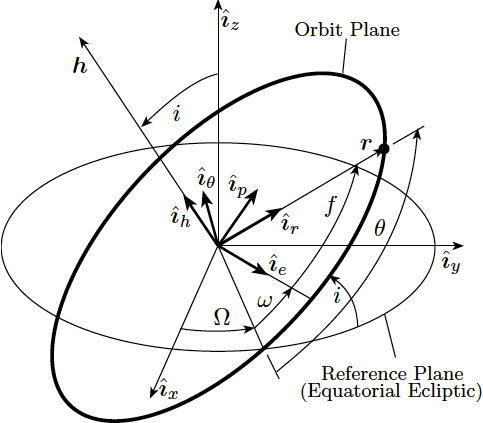
\includegraphics[width=0.3\textwidth]{Figures/orb_elem.png}
	\caption{Illustration of Keplerian Orbital Elements and Plane}\label{fig:OrbElem}
\end{figure} 
The mathematical methods for conversion vary depending on parameter values, specifically semimajor axis and eccentricity inputs. Outlined below are three cases for varying $a$ and $e$. Although the first case is supported when converting from orbital elements to Cartesian, it is not accurate for the reverse process and is considered a limitation of this module. The mathematical model is still briefly explained below but the first case is not tested. These cases all result in three-component position and velocity vectors.
\paragraph{Case 1 (\boldmath$e=1.0$, $a>0$):}
This case specifies a rectilinear, elliptical orbit. The first steps in obtaining position and velocity vectors is to find the orbit radius and the magnitude of rectilinear velocity. The orbit radius $r$ depends on the semimajor axis, eccentricity, and true anomaly. The velocity, as expected, depends on the orbit radius, semimajor axis, and gravitational constant. Both of these values can be found using the following equations:
\begin{equation}
r = a( 1-e \cos(f))
\end{equation}
\begin{equation}
v=\sqrt{\frac{2 \mu}{a(r-\mu)}}
\end{equation}
Fig. \ref{fig:OrbElem} illustrates the orbit frame \textit{O} with components $\{\bm{\hat{i}}_e$, $\bm{\hat{i}}_p$, $\bm{\hat{i}}_h\}$, the inertial frame \textit{N}$=\{\bm{\hat{i}}_x$, $\bm{\hat{i}}_y$, $\bm{\hat{i}}_z\}$, and the frame \textit{M} which tracks the position of the body with components $\{\bm{\hat{i}}_r$, $\bm{\hat{i}}_\theta$, $\bm{\hat{i}}_h\}$. For rectilinear orbits, the Euler angle set $\{\Omega$, $i$, $\omega\}$ relates the orientation of frame \textit{M} to \textit{N}, providing the ability to parameterize the direction cosine matrix and solve for position and velocity. This is shown by Eq. \ref{eq:3} below.

\begin{equation} \label{eq:3}
\bm{r} = r\begin{pmatrix}
\cos(\Omega)\cos(\omega)-\sin(\Omega)\sin(\omega)\cos(i) \\ \sin(\Omega)\cos(\omega)+\cos(\Omega)\sin(\omega)\cos(i) \\ \sin(\omega)\sin(i)
\end{pmatrix}
\end{equation}
The same parameterization is used when determining both position and velocity for a rectilinear orbit, giving
\begin{equation} \label{eq:4}
\bm{\dot{r}} = v\begin{pmatrix}
\cos(\Omega)\cos(\omega)-\sin(\Omega)\sin(\omega)\cos(i) \\ \sin(\Omega)\cos(\omega)+\cos(\Omega)\sin(\omega)\cos(i) \\ \sin(\omega)\sin(i)
\end{pmatrix}
\end{equation}

\paragraph{Case 2 (\boldmath $e=1.0$, $a<0$):} This case indicates a parabolic orbit, which naturally has an infinite semimajor axis. For computational purposes and to distinguish this case from a rectilinear orbit, the negative radius at periapsis will be used instead of an infinite semimajor axis. The radius is used to determine a semiparameter $p$, which describes the size of the orbit's conic section. These relationships are as follows:
\begin{equation} \label{eq:6}
r_p = -a
\end{equation}
\begin{equation} \label{eq:7}
p = 2r_p
\end{equation}
As with Case 1, the orbit radius, velocity magnitude, and parameterized direction cosine matrix are used to compute the Cartesian vectors. The radius and velocity  are determined largely using Kepler's first law, which gives the general trajectory equation shown here:

\begin{equation} \label{eq:8}
r = \frac{p}{1+e\cos(f)}
\end{equation}
For this case, the relationship between frames \textit{M} and \textit{N} uses the Euler angle set $\{\Omega$, $i$, $\theta\}$ where $\theta = \omega + f$ is the true latitude.
To find the position vector, $\theta$ is substituted for $\omega$ in the vector from Eq. \ref{eq:3}. This can be written as
\begin{equation}\label{eq:9}
\bm{r} = r\begin{pmatrix}
\cos(\Omega)\cos(\theta)-\sin(\Omega)\sin(\theta)\cos(i) \\ \sin(\Omega)\cos(\theta)+\cos(\Omega)\sin(\theta)\cos(i) \\ \sin(\theta)\sin(i)
\end{pmatrix}
\end{equation}
Taking the derivative of this equation gives the velocity vector, which implements angular momentum $h$ as shown in the following equations:
\begin{equation}\label{eq:10}
\bm{\dot{r}} = -\frac{\mu}{h}\begin{pmatrix}
\cos(\Omega)(\sin(\theta)+e\sin(\omega))+\sin(\Omega)(\cos(\theta)+e\cos(\omega))\cos(i) \\ \sin(\Omega)(\sin(\theta)+e\sin(\omega))+\cos(\Omega)(\cos(\theta)+e\cos(\omega))\cos(i) \\ -(\cos(\theta)+e\cos(\omega))\sin(i)
\end{pmatrix}
\end{equation}
\begin{equation} \label{eq:11}
h = \sqrt{\mu p}
\end{equation}
\begin{equation}\label{eq:12}
\bm{\dot{r}} = -\sqrt{\frac{\mu}{p}}\begin{pmatrix}
\cos(\Omega)(\sin(\theta)+e\sin(\omega))+\sin(\Omega)(\cos(\theta)+e\cos(\omega))\cos(i) \\ \sin(\Omega)(\sin(\theta)+e\sin(\omega))+\cos(\Omega)(\cos(\theta)+e\cos(\omega))\cos(i) \\ -(\cos(\theta)+e\cos(\omega))\sin(i)
\end{pmatrix}
\end{equation}
\paragraph{Case 3 (\boldmath$0<e<1.0$, $a>0$) or ($e>1.0$, $a<0$):}
This case applies to any scenario not included in cases 1 or 2, that is where eccentricity is bounded between 0 and 1.0 for a positive semimajor axis and greater than 1.0 for a negative semimajor axis.

The only difference between calculating Cartesian vectors in this case and the second is the method of determining the semiparameter, as to avoid a negative value. This is shown by the following equation:
\begin{equation}
p = a (1-e^2)
\end{equation}
Eq. \ref{eq:8} - \ref{eq:12} remain the same for this case and can be used to find the Cartesian vectors. From Eq. \ref{eq:11}, it is clear that the orbit's angular momentum is proportional to $\sqrt{p}$, resulting in an imaginary angular momentum when given a negative semiparameter. This is why limits are set for $a$ and $e$ in this case.

\subsubsection{Cartesian to Elements}
Since Keplerian orbital elements are the parameters primarily used to identify orbits, conversion from Cartesian vectors to these elements is an important function. That is, converting position and velocity vectors to the six elements previously discussed ($a$, $e$, $i$, $\Omega$, $\omega$, $f$). This conversion requires the input of a position and velocity vector, both consisting of three components, and a gravitational constant $\mu$, like the previous conversion. Presented below is the mathematical process for converting from Cartesian to orbital elements.

Like the reverse process, this conversion has several cases, this time depending on the semimajor axis, eccentricity, \textit{and} inclination. This means that the cases do not present themselves until those parameters are to be defined. That said, the first step is to calculate the position and velocity magnitudes, $r_0$ and $v_0$. Magnitudes of position and velocity can be determined from the vectors as follows:
\begin{equation}
r_0 = \sqrt{\bm{r} \cdot \bm{r}}
\end{equation}
\begin{equation}
v_0 = \sqrt{\bm{\dot{r}} \cdot \bm{\dot{r}}}
\end{equation}
Since eccentricity relies only on position, velocity, and the gravity constant $\mu$, it can now be calculated. The equation for the eccentricity vector is
\begin{equation} \label{eq:18}
\bm{e} = \frac{(v_0^2-\frac{\mu}{r_0})\bm{r} - (\bm{r} \cdot \bm{\dot{r}})\bm{\dot{r}}}{\mu}
\end{equation}
Once the magnitude $e$ is found, it can be used with $r_0$ and $v_0$ to find the semimajor axis. However, this is when unique cases begin to emerge. They are defined below.\\

\underline{Semimajor Axis Case 1 (non-parabolic finite $a$):}\\
For non-parabolic orbits, the semimajor axis is given by the following energy equation:
\begin{equation}
a = (\frac{2}{r_0}-\frac{v_0^2}{\mu})^{-1}
\end{equation}

\underline{Semimajor Axis Case 2 (parabolic infinite $a$):}\\
For parabolic orbits, the semimajor axis is infinite, so a semiparameter is used instead for computational purposes.
\begin{equation}
a = - \frac{p}{2}
\end{equation}
The semiparameter $p$ is given by
\begin{equation}
p = \frac{h^2}{\mu}
\end{equation}
To find the inclination of the orbit, it is neccessary to first calculate the angular momentum. In vector form, the angular momentum is calculated with a cross product as shown below.
\begin{equation}
\bm{h} = \bm{r} \times \bm{\dot{r}}
\end{equation}
This vector is normalized and the magnitude is obtained with the following equations:
\begin{equation}
h = \sqrt{\bm{h} \cdot \bm{h}}
\end{equation}
After finding angular momentum, it can be used to determine the inclination of the orbit plane. This inverse cosine expression involves only the second term of the angular momentum vector, denoted by $\bm{\hat{h}}_2$, and the magnitude. It can be written as
\begin{equation}
i = \cos^{-1}(\frac{\bm{\hat{h}}_2}{h})
\end{equation}
In addition to the inclination angle, it is important to find the line of nodes. The line of nodes is necessary, specifically, to identify inclined orbits and is not useful for equatorial orbits. First, set up a unit vector $u$ to cross with the angular momentum vector, resulting in a line of nodes vector, and then calculate the magnitude.
\begin{equation}
\bm{u} = <0, 0, 1.0>
\end{equation}
\begin{equation}
\bm{n} = \bm{u} \times \bm{h}
\end{equation}
\begin{equation}
n = \sqrt{\bm{n} \cdot \bm{n}}
\end{equation}
The vector $\bm{n}$ consists of three components, which will be referred to as $\bm{\hat{n}}_1$, $\bm{\hat{n}}_2$, and $\bm{\hat{n}}_3$. This provides the final parameter needed to find the remaining orbital elements and, ultimately, the orbit type. The methods for determining the ascending node, argument of periapsis, and true anomaly angles depend on the eccentricity and inclination, introducing the four cases presented below.
\paragraph{Case 1 (Non-circular, inclined orbit):}
A non-circular orbit is specified with $e>0$ and an inclined orbit has an inclination $i>0$. Since it is for inclined orbits, this case depends on the line of nodes. Each remaining orbital element is calculated with cosine expressions, so depending on the sign of the line of nodes components, the angles may need to be adjusted by a $2\pi$ radians. Subcases are shown for these adjustments.
\begin{equation} \label{eq:29}
\Omega = 
\begin{cases}
\cos^{-1}(\frac{\bm{\hat{n}}_1}{n}) & \bm{\hat{n}}_2 > 0\\
2\pi - \cos^{-1}(\frac{\bm{\hat{n}}_1}{n}) & \bm{\hat{n}}_2 < 0
\end{cases}
\end{equation}
Calculating the ascending node requires the eccentricity vector found previously in Eq. \ref{eq:18}.
\begin{equation} \label{eq:30}
\omega = 
\begin{cases}
\cos^{-1}(\frac{\bm{n} \cdot \bm{e}}{n e}) & \bm{\hat{n}}_3 > 0\\
2\pi - \cos^{-1}(\frac{\bm{n} \cdot \bm{e}}{n e}) & \bm{\hat{n}}_3 < 0
\end{cases}
\end{equation}
Finding the true anomaly also requires the eccentricity vector as well as the position vector, its magnitude, and the velocity vector. 
\begin{equation} \label{eq:31}
f =
\begin{cases}
\cos^{-1}(\frac{\bm{e} \cdot \bm{r}}{e r_0}) & \bm{r} \cdot \bm{\dot{r}} > 0\\
2\pi - \cos^{-1}(\frac{\bm{e} \cdot \bm{r}}{e r_0}) & \bm{r} \cdot \bm{\dot{r}} < 0
\end{cases}
\end{equation}
\paragraph{Case 2 (Non-circular, equatorial orbit):}
An equatorial orbit is specified with $i>0$. The true anomaly can still be calculated with Eq. \ref{eq:31} but the methods for finding the ascending node and argument of periapsis differ from those in the first case. An equatorial orbit has no ascending node, meaning
\begin{equation}
\Omega = 0
\end{equation}
It also uses the true longitude of periapsis, defining
\begin{equation}
\omega = 
\begin{cases}
\cos^{-1}(\frac{\bm{\hat{e}}_1}{n e}) & \bm{\hat{e}}_2 > 0 \\
2\pi - \cos^{-1}(\frac{\bm{\hat{e}}_1}{n e}) & \bm{\hat{e}}_2 < 0
\end{cases}
\end{equation}

\paragraph{Case 3 (Circular, inclined orbit):}
This case also differs from the first by two elements, the argument of periapsis and true anomaly. The ascending node can still be determined with Eq. \ref{eq:29}. A circular orbit has no argument of periapsis, so for this case
\begin{equation}
\omega = 0
\end{equation}
The true anomaly substitutes eccentricity for the line of nodes vector and magnitude in Eq. \ref{eq:31}. It also gets adjusted by $2\pi$ depending on the sign of the position vector's third component, denoted by $\bm{\hat{r}}_3$. This results in the following equation
\begin{equation}
f=\begin{cases}
\cos^{-1}(\frac{\bm{n} \cdot \bm{r}}{n r_0}) & \bm{\hat{r}}_3 > 0\\
2\pi - \cos^{-1}(\frac{\bm{n} \cdot \bm{r}}{n r_0}) & \bm{\hat{r}}_3 < 0
\end{cases}
\end{equation}
\paragraph{Case 4 (Circular, equatorial orbit):}
This case is a combination of the previous two, where the orbit has neither an ascending node or an argument of periapsis, giving
\begin{equation}
\Omega = 0
\end{equation}
\begin{equation}
\omega = 0
\end{equation}
Due to the eccentricity and the inclination both being equal to zero, the true anomaly also changes. It now only depends on the position vector's first and second terms, $\bm{\hat{r}}_1$ and $\bm{\hat{r}}_2$, and its magnitude. This can be written as
\begin{equation}
f=\begin{cases}
\cos^{-1}(\frac{\bm{r}_1}{r_0}) & \bm{\hat{r}}_2 > 0\\
2\pi - \cos^{-1}(\frac{\bm{r}_1}{r_0}) & \bm{\hat{r}}_2 < 0
\end{cases}
\end{equation}
Lastly, to ensure the appropriate value is used for the true anomaly, it should be checked whether the orbit is parabolic or hyperbolic. For both of these orbit types, a true anomaly greater than $\pi$ and less then $2\pi$ would mean the body is outside of the orbit. Thus, a limit must be applied to the true anomaly for parabolic and hyperbolic orbits, as shown below. The sign of $f$ remains the same after changing the magnitude.
\begin{equation}
f = 
\begin{cases}
\pm 2\pi & \quad |e|\geq 1.0 \quad \textrm{and} \quad |\pm f|>\pi
\end{cases}
\end{equation}
